\begin{mybilan}
	\begin{itemize}
		\item Un atome est constitué d'un \kw{noyau} au centre et d'\kw{électrons} qui se déplacent autour.
		\item Le noyau est composé de \kw{nucléons (protons et neutrons)}.
		\item Le \kw{numéro atomique Z} d'un élément chimique est le nombre de protons dans son noyau.
		\item Un atome possède autant de protons (chargés positivement) que d'électrons (chargés négativement), il est \kw{électriquement neutre}.
		\item Deux atomes d'un même élément possèdent le même nombre de protons mais peuvent avoir un nombre de neutrons différent : ce sont des \kw{isotopes}.
	\end{itemize}
	
	\begin{center}
		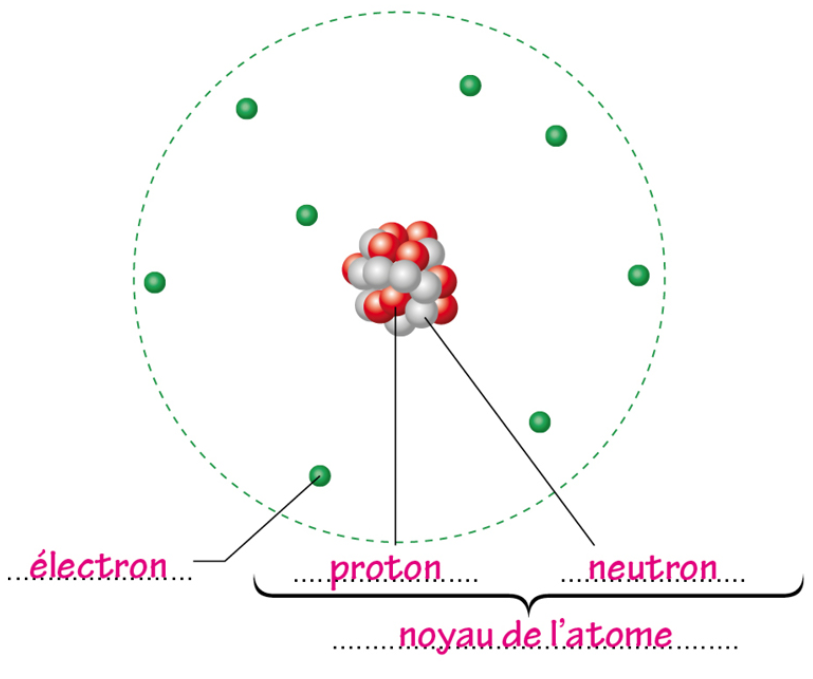
\includegraphics[scale=0.45]{struct_atome}
	\end{center}
	

\end{mybilan}
